% appendix/questions/time.tex
% mainfile: ../../perfbook.tex
% SPDX-License-Identifier: CC-BY-SA-3.0

\section{What Time Is It?}
\label{sec:app:questions:What Time Is It?}

\begin{figure}[tb]
\centering
\resizebox{2.6in}{!}{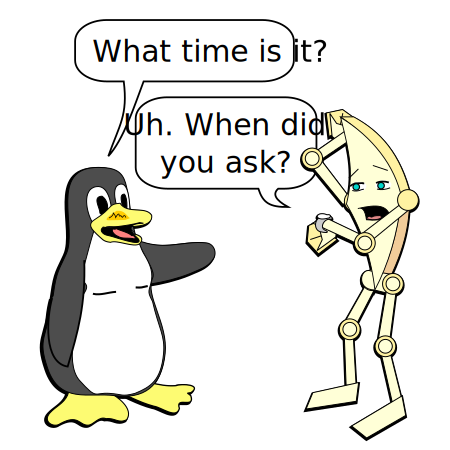
\includegraphics{cartoons/r-2014-What-time-is-it}}
\caption{What Time Is It?}
\ContributedBy{Figure}{fig:app:questions:What Time Is It?}{Melissa Broussard}
\end{figure}

멀티코어 컴퓨터 시스템에서의 시간 관리에서의 핵심적 문제가
\cref{fig:app:questions:What Time Is It?} 로 그려져 있습니다.
한가지 문제는 시간을 읽는데 시간이 걸린다는 겁니다.
어떤 명령은 하드웨어 시계를 읽을거고, 이 읽기 오퍼레이션을 완료하기 위해
off-core (더 나쁜 경우 off-socket) 으로 나가야 할수도 있습니다.
읽혀진 값에 대한 어떤 연산을 해야할 수도 있는데, 예를 들어 요구된 포맷으로
변환하기 위해, network time protocol (NTP) 조정을 위해, 등등이 있겠습니다.
그러니 결국 반환된 시간은 초래된 시간 간격의 시작, 끝, 또는 그 사이 어디에
맞춰져 있을까요?

더 나쁜게, 시간을 읽는 쓰레드는 인터럽트 당하거나 preemption 당할 수도
있습니다.
더 나아가, 시간을 읽는 시점과 그 시간의 실제 사용 사이에 어떤 연산이 있을
겁니다.
이 두개의 가능성 모두 이 불확정 시간을 늘립니다.

\iffalse

A key issue with timekeeping on multicore computer systems is illustrated
by \cref{fig:app:questions:What Time Is It?}.
One problem is that it takes time to read out the time.
An instruction might read from a hardware clock, and might
have to go off-core (or worse yet, off-socket) to complete
this read operation.
It might also be necessary to do some computation on the value read out,
for example, to convert it to the desired format, to apply network time
protocol (NTP) adjustments, and so on.
So does the time eventually returned correspond to the beginning of
the resulting time interval, the end, or somewhere in between?

Worse yet, the thread reading the time might be interrupted or preempted.
Furthermore, there will likely be some computation between reading out
the time and the actual use of the time that has been read out.
Both of these possibilities further extend the interval of uncertainty.

\fi

한가지 방법은 시간을 두번 읽고 타임스탬프가 만들어지는 이 오퍼레이션의 각 방향
중 하나에 있는, 이 두 읽기의 수치적 중간값을 사용하는 것입니다.
그럼 이 두 읽기 사이의 차이는 중간의 오퍼레이션이 수행된 시간의 불확정성의
측정값이 됩니다.

물론, 많은 경우 정확한 시간이 필요합니다.
예를 들어, 인간 사용자의 이익을 위한 시간을 출력하는 경우, 우린 내부의
하드웨어와 소프트웨어 지연이 쓸모없어지는 인간의 느린 반사속도에 기댈 수
있습니다.
비슷하게, 어떤 서버가 클라이언트로의 응답에 시간을 기록해야 한다면, 요청의
도착과 응답의 전송 사이 어느 시간이든 잘 동작할 겁니다.

\iffalse

One approach is to read the time twice, and take the arithmetic mean
of the two readings, perhaps one on each side of the operation being
timestamped.
The difference between the two readings is then a measure of uncertainty
of the time at which the intervening operation occurred.

Of course, in many cases, the exact time is not necessary.
For example, when printing the time for the benefit of a human user,
we can rely on slow human reflexes to render internal hardware and
software delays irrelevant.
Similarly, if a server needs to timestamp the response to a client, any
time between the reception of the request and the transmission of the
response will do equally well.

\fi

% @@@ Scheduling ticks

% @@@ Tickless operation

% @@@ Timers

% @@@ Current time, monotonic operation

% @@@ The many ways in which time can appear to go backwards

% @@@ Causality, the only real time in SMP (or distributed) systems
